\section{Participation notes 2}
Participant: Student

\begin{itemize}
    \item \textbf{Have them read the code-example} - Participant did not have any problem reading the code.
    \item \textbf{Have them draw the structure} - Participant separated the two called functions into each their circle and added names to each of them. Participant then represented main as a square and drew arrows from main to each function and explained that they were function calls.
    \item \textbf{Have them submit the git URL} - Participant wrote into the git repository field and submitted without problem. Afterwards, the participant used mouse to navigate successfully.
    \item \textbf{Have them get the main() implementation} - Participant was able to find implementation of both main and other functions.
    \item \textbf{Participant visualization} \includepdf[pages={4}]{inc/generalAppendix/userStudies/participantsVisualization.pdf}
\end{itemize}